%\pagebreak
\section{Measurement setup}

\dropcap{O}{nce} the experimentalist has deemed their sample worthy of measuring, there are a few battles to be fought outside the cleanroom and in the measurement laboratory.

\subsection{Thermal energy and noise}

Temperature means that there are available excitations at a given energy, corresponding to a (thermal) frequency
\begin{align}
f_{th}=\frac{k_B T}{h}.
\end{align}
Below we give the thermal energies and frequencies corresponding to typical temperatures in our setups:
\begin{center}
\begin{tabular}{ccc}
	\hline \hline
	Temperature & Thermal frequency & Thermal energy \\ 
	\hline 
	\SI{300}{\kelvin} & \SI{6.25}{\tera\hertz} & \SI{25.9}{\milli\electronvolt} \\ 
	% \hline 
	\SI{50}{\kelvin} & \SI{1.04}{\tera\hertz} & \SI{4.3}{\milli\electronvolt} \\ 
	% \hline 
	\SI{4}{\kelvin} & \SI{83.3}{\giga\hertz} & \SI{345}{\micro\electronvolt} \\ 
	% \hline 
	\SI{100}{\milli\kelvin} & \SI{2}{\giga\hertz} & \SI{8.62}{\micro\electronvolt} \\ 
	% \hline 
	\SI{10}{\milli\kelvin} & \SI{208}{\mega\hertz} & \SI{862}{\nano\electronvolt} \\ 
	\hline \hline
\end{tabular}
\end{center}

In order to neglect the influence of thermal effects on our circuits and for the superconductor to be in its thermal ground state, it is absolutely necessary to operate the devices at temperatures $T \ll T_c$.
Since the superconducting gap voltages of \ce{NbTiN}, \ce{MoRe} and \ce{Al} are \SI{2.3}{\milli\electronvolt}, \SI{1.5}{\milli\electronvolt} and \SI{183}{\micro\electronvolt}, respectively, our experiments require access to the sub-Kelvin regime which is enabled by using dilution refridgerators.

However, even with thermal excitations supressed by thermally anchoring our devices to the milliKelvin stages of our dilution refridgerators, thermal noise from our setup propagating through the electrical connections necessary to probe our devices, can induce unwanted excitations which can severly hinder experiments.
The amplitude of such thermal noise current, voltage and power of a resistor are
\begin{align}
I_n &= \sqrt{\frac{4k_B T\Delta f}{R}} \\
V_n &= \sqrt{4k_B T R\Delta f} \\
P_n &= k_B T \Delta f \\
P_{dBm} &= 10\log_{10}(k_B T\Delta f)+30
\end{align}

For a measurement bandwidth of \SI{1}{\hertz} and a resistor of \SI{50}{\ohm}, this corresponds to the following values for temperatures typically used in our setup:

\begin{center}
\begin{tabular}{cccc}
	\hline \hline
	Temperature (\si{\kelvin}) & Noise power (\si{dBm}) & Noise voltage (\si{\pico\volt}) & Noise current (\si{\pico\ampere})\\ 
	\hline 
	300 & -174 & 910 & 18 \\ 
	% \hline 
	50 & -182 & 372 & 7 \\ 
	% \hline 
	4 & -193 & 105 & 2 \\ 
	% \hline 
	0.1 & -209 & 16.6 & 0.3 \\ 
	% \hline 
	0.01 & -219 & 5.3 & 0.1 \\ 
	\hline \hline
\end{tabular}
\end{center}

Moreover, current and voltage fluctuations originating from room temperature electronics can carry the typical \SI{50}{\hertz} interference (also dubbed \textit{mains hum}), along with other, high-frequency, components.
In our lab, we suppress the mains hum by physically separating any electronic equipment powered by the \SI{50}{\hertz} power system from our DC electronics.
Our DC electronics, the IVVI rack, is home-made at \textit{DEMO}\footnote{Dienst Elektronische en Mechanische Ontwikkeling, \url{https://www.tudelft.nl/demo/}} of TU Delft.
\begin{itemize}
	\item 50 Hz
	\item other sources of electronic noise
	\item battery powered and separated grounds, including measurement?
	\item low pass filters
\end{itemize}

The detailed recipe for making the copper powder filters can be found in appendix \ref{app:copperpowder}.

\begin{figure}
	\centering
	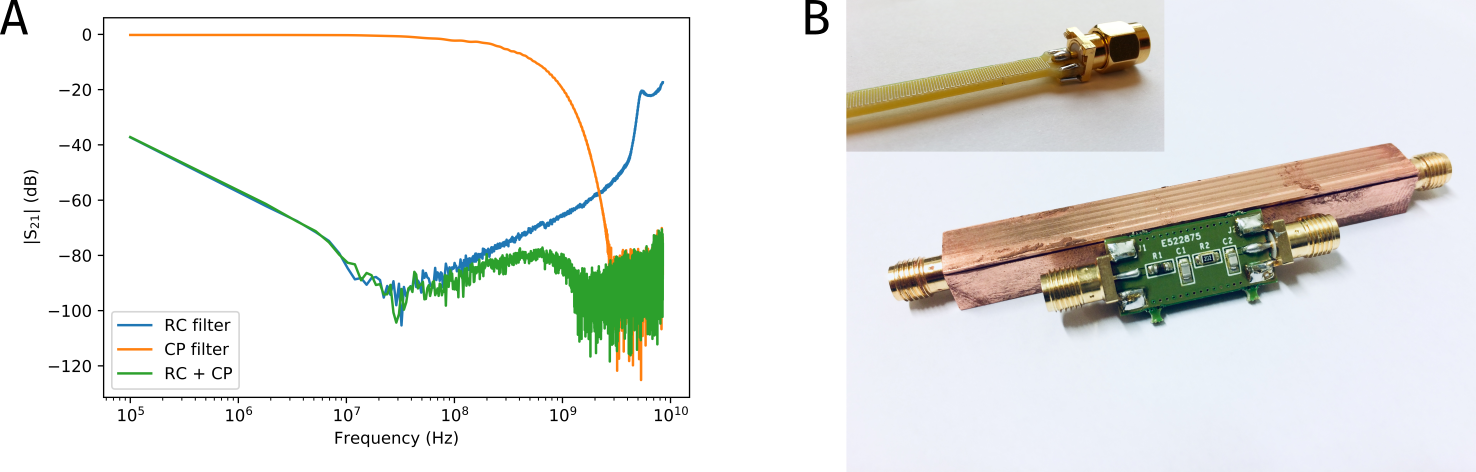
\includegraphics[]{{chapter-experimental-methods/figs-setup/noise_filter.svg}.png}
	\caption{
		\textbf{Electronic noise reduction using low-pass filters.}
		\textbf{A,} Measured transfer function of individual homemade copper powder and two-stage RC filters.
		The cut-off frequency for the RC filters is approximately \SI{30}{kHz}, while high-frequency noise leaks through above \SI{20}{MHz}.
		The copper powder filters significantly suppress frequencies above \SI{100}{MHz} and above.
		\textbf{B,} Photograph of a two-stage RC filter of SMD 0812 elements and a fully assembled copper powder filter.
		Inset, copper powder filter PCB with connector, without enclosure.
		The PCB trace is approximately \SI{50}{\centi\meter} long.
	}
	\label{fig:filter}
\end{figure}

\subsection{Fridge wiring}

\begin{figure}
	\centering
	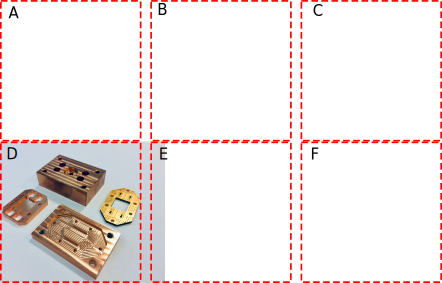
\includegraphics[]{{chapter-experimental-methods/figs-packaging/wiring.svg}.png}
	\caption{
		\textbf{Cryogenic fridge wiring.}
		\textbf{A,} Inside view of a Bluefors LD dry dilution refridgerator.
		\textbf{B,} Photograph of a four-port PCB mounted on a copper block with rails.
		\textbf{C,} Fully enclosed sample mounted inside of a hand-wound magnet and bolted to the millikelvin stage of the dilution refridgerator.
	}
	\label{fig:wiring}
\end{figure}

All measurements presented in this thesis were performed in dry dilution refridgerators from \textit{Oxford Instruments} or \textit{Bluefors Oy} at millikelvin temperatures.

\begin{itemize}
	\item noise temperature calculation a la Bluefors
	\item pictures
\end{itemize}

